
%%%%%%%%%%

\begin{frame}{\vskip -0.2cm \large The optimization problem behind classification trees}

\Large
\begin{center}
\pause
Minimize objective function (a.k.a. cost function)
\end{center}

\large
\begin{itemize}
\item
	\pause
	Domain (a.k.a. hypothesis class)
	\vskip -0.1cm
	{\scriptsize\begin{equation*}
	\pause
	\left\{\begin{array}{c}
		\overset{{\color{white}.}}{\textnormal{recursive binary}} \\
		\textnormal{partitioning trees}
	\end{array}\right\}
	\pause
	\quad\sim\quad
	\left\{\begin{array}{c}
		\overset{{\color{white}.}}{\textnormal{piecewise constant functions}} \\
		\textnormal{resulting from} \\
		\textnormal{recursive binary partitioning}
	\end{array}\right\}
	\end{equation*}}

\item
	\pause
	Actual form of the objective function
	\pause
	\vskip -0.1cm
	{\footnotesize\begin{equation*}
	\textnormal{tree impurity}
	\;=\;
		\textnormal{weighted average of leaf impurities}
	\end{equation*}}

\item
	\pause
	Algorithm (greedy, iterative)
	\begin{itemize}
	\item
		\pause
		{\footnotesize At each step, select ``best'' node to split and how best to split it: CART}
	\item
		\pause
		{\footnotesize Pruning: prune back fully split tree to mitigate for overfitting}
	\end{itemize}
\end{itemize}

\end{frame}
\normalsize

%%%%%%%%%%

\begin{frame}{\vskip -0.2cm \large The optimization problem behind classification trees}

\large
\begin{itemize}
\item
	{\Large Domain of objective function} {\small (a.k.a. hypothesis class)}
	{\scriptsize\begin{equation*}
	\left\{\begin{array}{c}
		\overset{{\color{white}.}}{\textnormal{recursive binary}} \\
		\textnormal{partitioning trees}
	\end{array}\right\}
	\quad\sim\quad
	\left\{\begin{array}{c}
		\overset{{\color{white}.}}{\textnormal{piecewise constant functions}} \\
		\textnormal{resulting from} \\
		\textnormal{recursive binary partitioning}
	\end{array}\right\}
	\end{equation*}}
	\begin{center}
	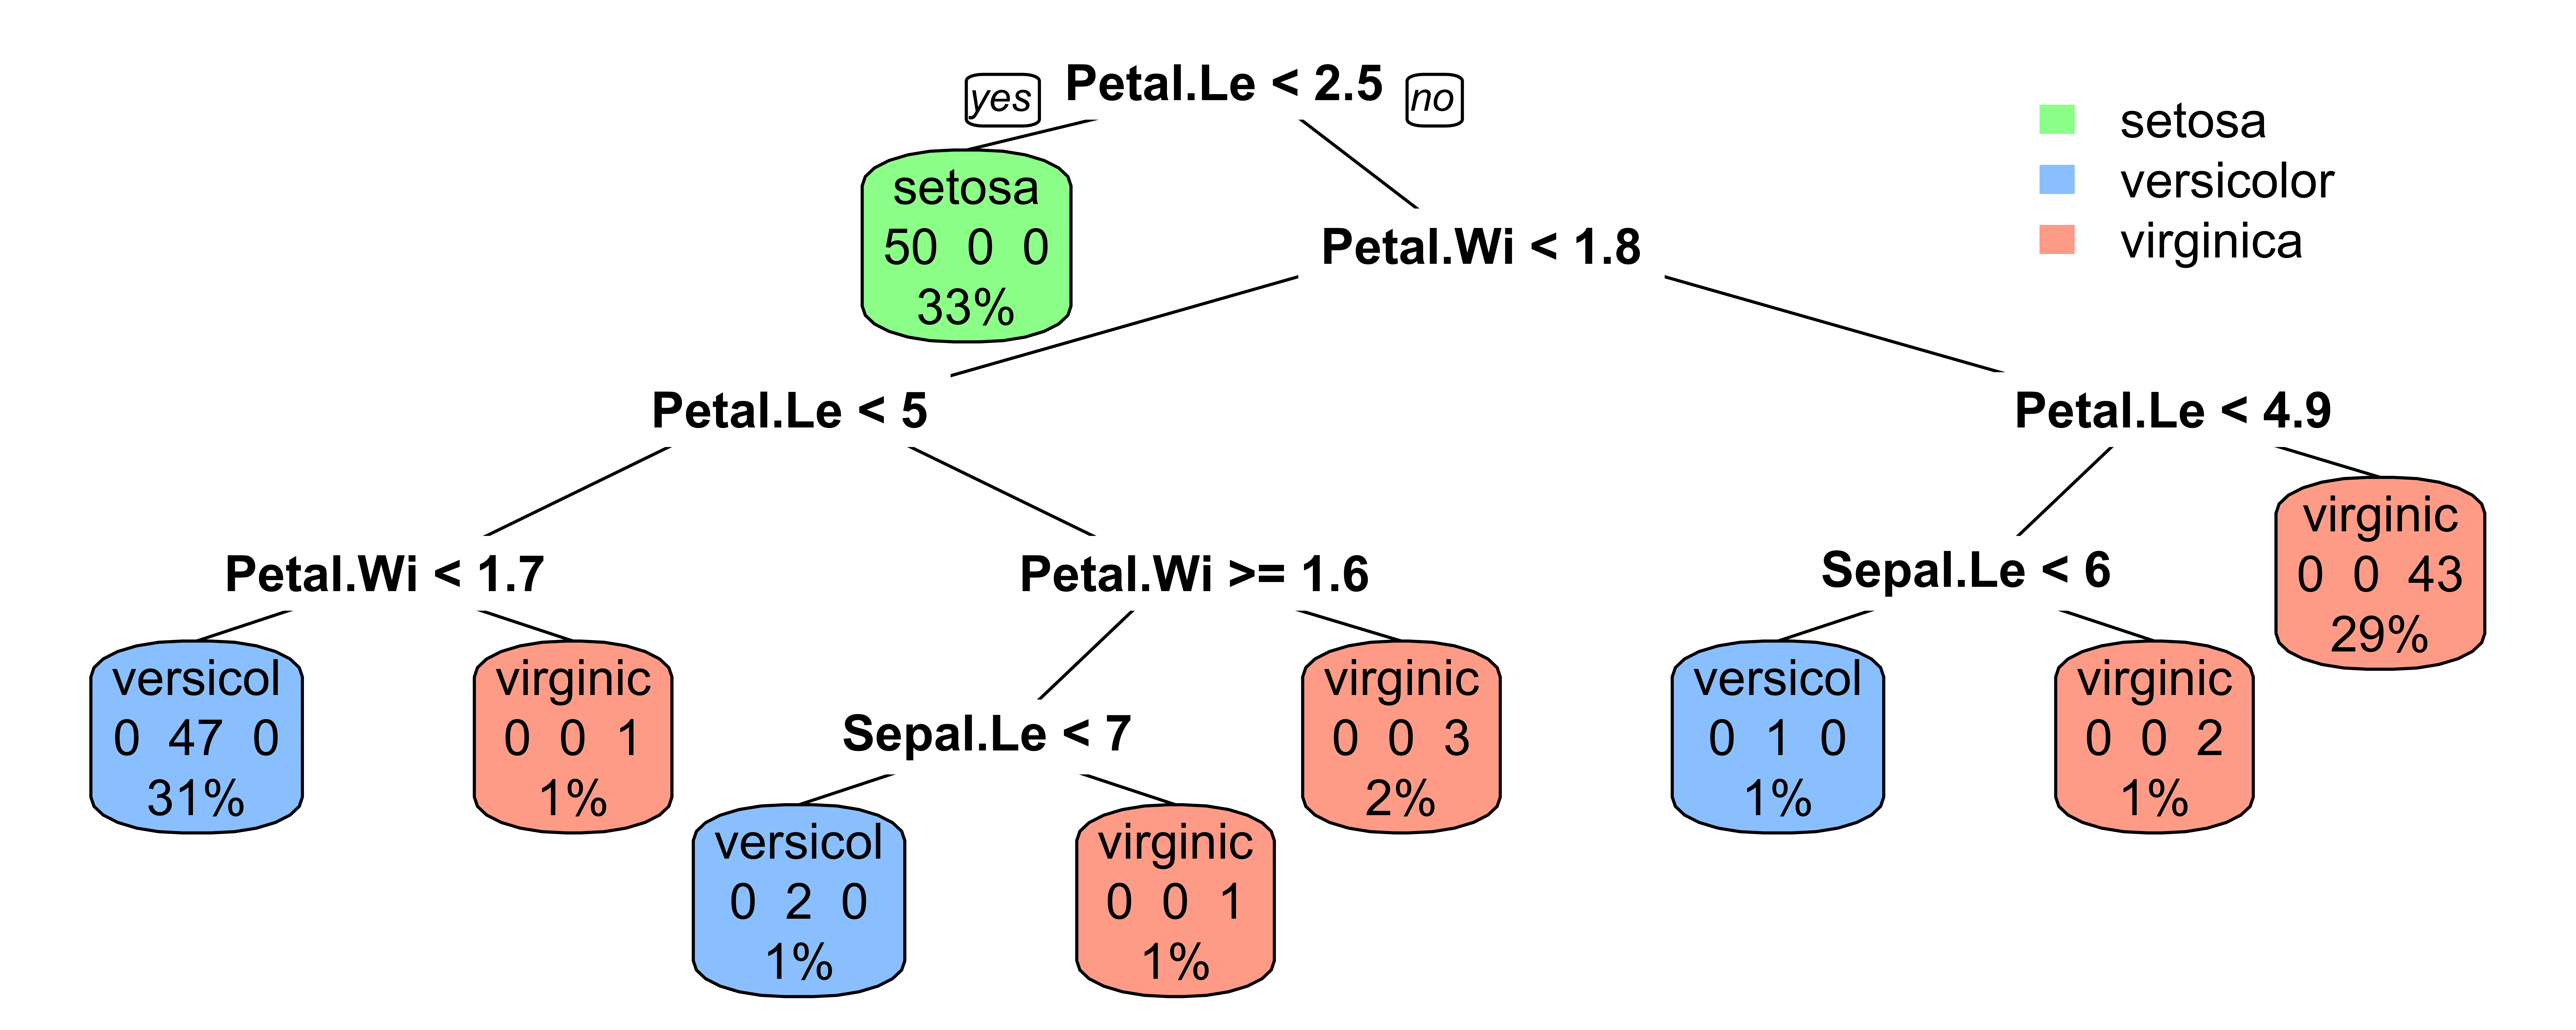
\includegraphics[width=2.5cm,height=3.5cm]{graphics/plot-rpart.png}
	\quad\quad\quad\quad\;\;
	\includegraphics[width=2.5cm,height=3.25cm]{graphics/plot-regression-surface.png}
	\;\;{\color{white}1}
	\end{center}
\end{itemize}


\end{frame}
\normalsize

%%%%%%%%%%

\begin{frame}{\vskip -0.2cm \large The optimization problem behind classification trees}

\small

\begin{multicols}{2}

	\begin{center}
	\begin{minipage}{4.5cm}
	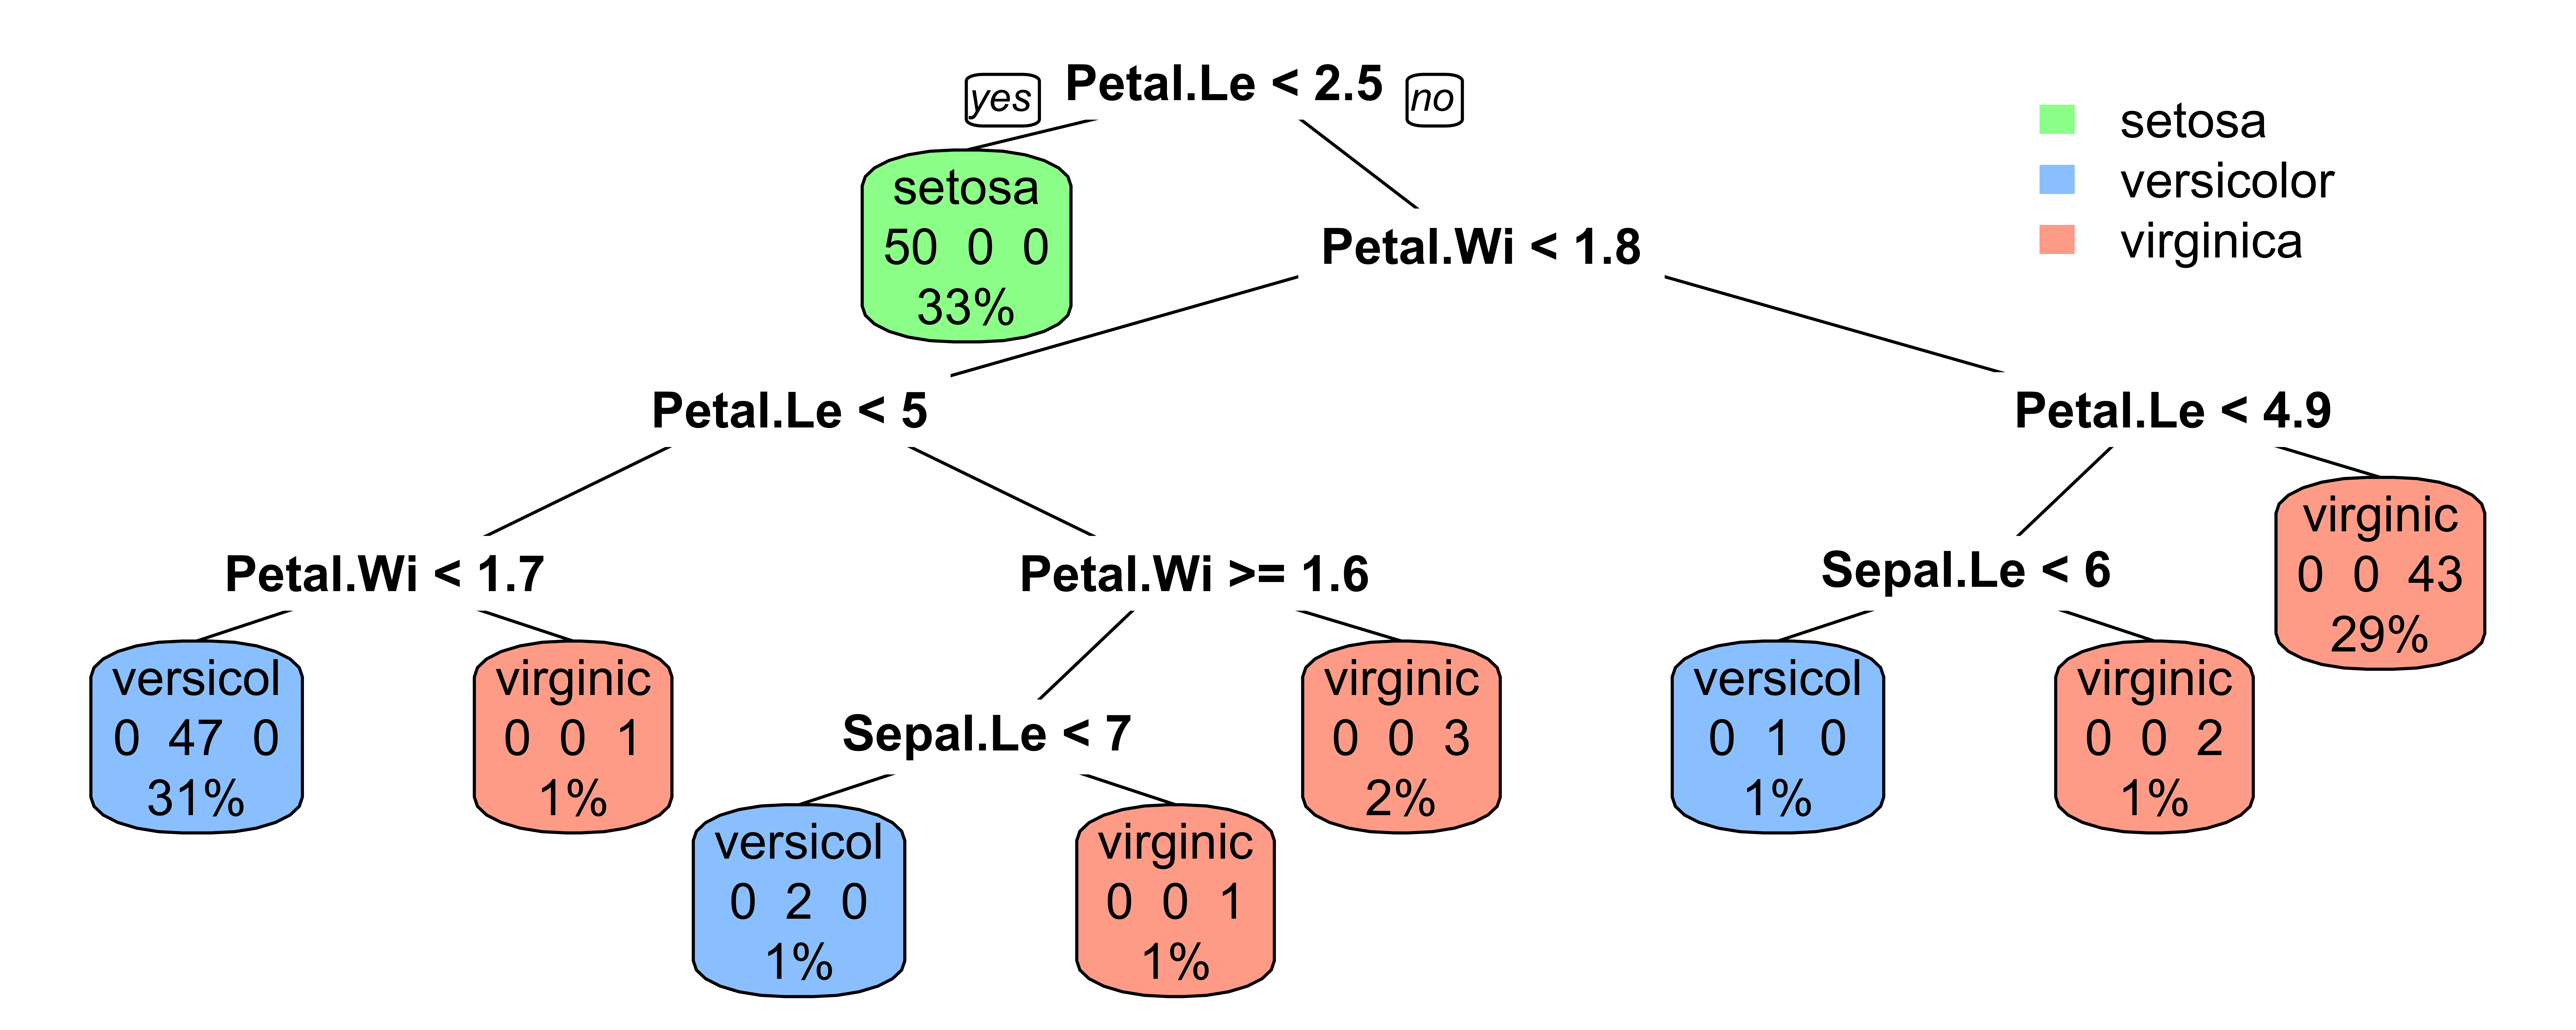
\includegraphics[width=4.5cm,height=6.25cm]{graphics/plot-rpart.png}
	\end{minipage}
	\end{center}

\columnbreak

	\begin{flushleft}
	\begin{minipage}{6.0cm}
	\vskip -0.3cm
	\begin{itemize}
	\item
		{\Large Objective function}
		\vskip 0.3cm
		\begin{center}\textbf{Tree Impurity given Data}\end{center}
		\begin{equation*}
		I(T\,\vert D)
		\; =
			\underset{l\,\in\,\textnormal{Leaves}(T)}{\sum}\!\!
			P(X \!\in\! l\,) \cdot I(l\,\vert D)
		\end{equation*}
		{\scriptsize where}
		{\scriptsize\begin{eqnarray*}
		P(X \!\in\! l\,) &=& \left(\!\!\!\begin{array}{c}
			\textnormal{probability of a}
			\\
			\textnormal{randomly drawn unit}
			\\
			\textnormal{to reach leaf $l$}
			\end{array}\!\!\!\!\right)
		\\
		I(l\,\vert D) &=& \left(\!\!\begin{array}{c}
			\textnormal{impurity of leaf $l$}
			\\
			\textnormal{given data $D$}
			\end{array}\!\!\right)
		\end{eqnarray*}}
		{\scriptsize Common choices for $I(l\,\vert D)$:}
		\begin{center}
		\vskip -0.2cm
		Entropy,\;
		Gini Impurity
		\end{center}
	\end{itemize}
	\end{minipage}
	\end{flushleft}

\end{multicols}

\end{frame}
\normalsize

%%%%%%%%%%

\begin{frame}{\vskip -0.2cm \large Objective function: Tree Impurity given Data}

\vskip -0.3cm

\begin{eqnarray*}
\pause
I(T\,\vert D)
& = &
	\underset{l\,\in\,\textnormal{Leaves}(T)}{\sum}\!\!
	{\color{red}P(X \!\in\! l\,)} \cdot I(l\,\vert D)
\\
\pause
& \approx &
	\underset{l\,\in\,\textnormal{Leaves}(T)}{\sum}
	{\color{red}\widehat{p}(X \!\in\! l\,)} \cdot I(l\,\vert D)
\pause
\;\; = \;\;
	\underset{l\in\textnormal{Leaves}(T)}{\sum}
	{\color{red}\dfrac{\overset{n}{\underset{i=1}{\sum}}\,I_{\{x_{i} \in l\}}}{n}} \cdot I(l\,\vert D)
\end{eqnarray*}

\small
\begin{equation*}
\pause
I(l\,\vert D)
\;\; = \;\;
\left\{\begin{array}{ccl}
\pause
\textnormal{Entropy}
& := &
	\textnormal{\scriptsize$-\;\overset{C}{\underset{y=1}{\sum}}\;\,
	\widehat{p}(Y=c\,\vert X\in l\,) \cdot \log\,\widehat{p}(Y=c\,\vert X\in l\,)$}
\\
\pause
\textnormal{Gini Impurity}
& := &
	\textnormal{\scriptsize$+\;\overset{C}{\underset{y=1}{\sum}}\;\,
	\widehat{p}(Y=c\,\vert X\in l\,) \cdot
	\left(\overset{{\color{white}.}}{1}\,-\,\widehat{p}(Y=c\,\vert X\in l\,)\right)$}
\end{array}\right.
\end{equation*}

\pause
\vskip -0.5cm

\footnotesize
\begin{equation*}
\widehat{p}(Y=c\,\vert X\in l\,)
\;\; := \;\;
	\left.\overset{n}{\underset{i=1}{\sum}}\; I_{\{x_{i}\in l, y_{i} = c\}} \right\slash
	\overset{n}{\underset{i=1}{\sum}}\; I_{\{x_{i}\in l\}}
\end{equation*}

\end{frame}
\normalsize

%%%%%%%%%%

\begin{frame}{\vskip -0.2cm \Large Impurity metrics: Entropy \& Gini Impurity}

\vskip -0.2cm
\tiny
\begin{equation*}
I(l\,\vert D)
\;\; = \;\;
\left\{\begin{array}{ccl}
\textnormal{Entropy}
& := &
	\textnormal{\tiny$-\;\overset{C}{\underset{y=1}{\sum}}\;\,
	\widehat{p}(Y=c\,\vert X\in l\,) \cdot \log\,\widehat{p}(Y=c\,\vert X\in l\,)$}
\\
\textnormal{Gini Impurity}
& := &
	\textnormal{\tiny$+\;\overset{C}{\underset{y=1}{\sum}}\;\,
	\widehat{p}(Y=c\,\vert X\in l\,) \cdot
	\left(\overset{{\color{white}.}}{1}\,-\,\widehat{p}(Y=c\,\vert X\in l\,)\right)$}
\end{array}\right.
\end{equation*}

\begin{center}
\vskip -0.2cm
\includegraphics[height=6.0cm]{graphics/plot-impurity-metrics.png}
\end{center}

\end{frame}
\normalsize

%%%%%%%%%%
